\documentclass[border=2mm]{standalone}
\usepackage{tikz}
\usetikzlibrary{calc,patterns,angles,quotes}
\begin{document}
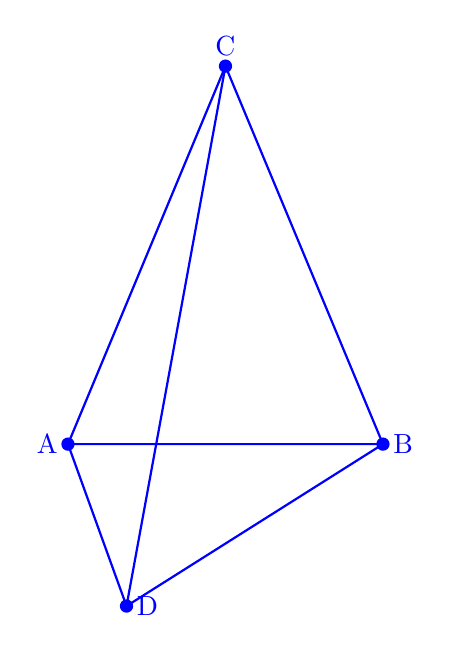
\begin{tikzpicture}[scale=0.8, blue, thick]
  \coordinate (A) at (0,0,0);
  \coordinate (B) at (5,0,0);
  \coordinate (C) at (2.5,6,0); % 2.5 = 5/2, 4.33 ≈ 5√3/2
  \coordinate (D) at (2.5,-1,4.08); % Trọng tâm tam giác ABC là (2.5, 4.33/3≈1.443), h ≈ 4.08

  \draw (A) -- (B) -- (C) -- cycle;
  \draw (A) -- (D);
  \draw (B) -- (D);
  \draw (C) -- (D);

  \fill[blue] (A) circle (3pt) node[left] {A};
  \fill[blue] (B) circle (3pt) node[right] {B};
  \fill[blue] (C) circle (3pt) node[above] {C};
  \fill[blue] (D) circle (3pt) node[right] {D};
\end{tikzpicture}
\end{document}